%-----------------------------------------
% Note: Use pdflatex to process this file.
%-----------------------------------------

%\documentclass{article}
\documentclass{hitec}
\usepackage{color,soul}

\usepackage{setspace}
\usepackage{graphicx}
\usepackage{moreverb}    % Defines {listing} environment.
\usepackage{amsmath, amsthm, amssymb, amsbsy, mathtools}
\usepackage{alltt}
\usepackage{rotating}
\usepackage{subcaption}
\usepackage{xspace}
\usepackage[section]{placeins}   % For preventing floats from floating to end of chapter.
\usepackage{longtable}   % For splitting long vertical tables into pieces
\usepackage{index}
\usepackage{multirow}
\usepackage{booktabs}    % For table layouts
\usepackage{yhmath}      % For widehat
\usepackage{xcolor}      % Needed for listings package.
\usepackage{listings}
\usepackage[T1]{fontenc}   % so _, <, and > print correctly in text.
\usepackage[strings]{underscore}    % to use "_" in text
\usepackage[pdftex,colorlinks=true,bookmarksnumbered=true]{hyperref}   % Must be last package!

\definecolor{light-gray}{gray}{0.95}
\lstset{backgroundcolor=\color{light-gray}}
\lstset{xleftmargin=0cm}
\lstset{framexleftmargin=0.3em}
%\lstset{basicstyle = \ttfamily\fontsize{11}{11}\selectfont} 
\lstset{basicstyle = \small}
\lstnewenvironment{code}{}{}

%---------------------------------------------------------------------------------

\definecolor{lightestgray}{gray}{0.99}
\sethlcolor{lightestgray}
\soulregister{\texttt}{1}
\newcommand\dottcmd[1]{\hl{\em#1}\endgroup}
%\newcommand\dottcmd[1]{{#1}\endgroup}
\newcommand{\vn}{\begingroup\catcode`\_=11 \catcode`\%=11 \dottcmd}
\newcommand{\ts}{\vn{tune_scan}\xspace}
\newcommand{\Newline}{\hfil \\}
\newcommand{\sref}[1]{$\S$\ref{#1}}
\newcommand{\Th}{$^{th}$\xspace}

%---------------------------------------------------------------------------------

\renewcommand{\textfraction}{0.1}
\renewcommand{\topfraction}{1.0}
\renewcommand{\bottomfraction}{1.0}

\settextfraction{0.9}  % Width of text
\setlength{\parindent}{0pt}
\setlength{\parskip}{1ex}
%\setlength{\textwidth}{6in}
\newcommand{\Section}[1]{\section{#1}\vspace*{-1ex}}

\newenvironment{display}
  {\vspace*{-1.5ex} \begin{alltt}}
  {\end{alltt} \vspace*{-1.0ex}}

%%% Table of Contents spacing.
\makeatletter
\renewcommand{\l@section}{\@dottedtocline{1}{1.5em}{3.3em}}
\renewcommand{\l@subsection}{\@dottedtocline{2}{3.8em}{4.2em}}
\renewcommand{\l@figure}{\@dottedtocline{1}{1.5em}{3.3em}}
\renewcommand{\l@table}{\@dottedtocline{1}{1.5em}{3.3em}}
\makeatother

%---------------------------------------------------------------------------------

\title{Tune Scan Program}
\author{}
\date{David Sagan \\ November 1, 2023}
\begin{document}
\maketitle

\tableofcontents

%---------------------------------------------------------------------------------

\Section{Introduction} 
\label{s:intro}

A \vn{tune scan} is a way of examining resonances which involves plotting a resonance related beam
parameter such as the beam size or the beam lifetime as a function of the transverse $Q_a$ and $Q_b$
tunes.  A scan can be done in an actual machine or in simulation which is what \ts program documented here
does. Since lifetimes can be tricky and time intensive to calculate, the \ts program uses variations in the
amplitude of a tracked particle as the indicator for resonance.

The \ts program is built atop the Bmad software toolkit \cite{b:bmad}. The Bmad toolkit is a
library, developed at Cornell, for the modeling relativistic charged particles in storage rings and
Linacs, as well as modeling photons in x-ray beam lines.

The \ts program comes with the ``Bmad Distribution'' which is a package which contains Bmad along with
a number of Bmad based programs. See the Bmad web site for more details.

The \ts program comes in two versions: 
\begin{code}
tune_scan      ! Single threaded version.
tune_scan_mpi  ! MPI threaded version.
\end{code}
The first version is a single threaded version and the second is a multi-threaded version using MPI.

[Note to Bmad Distribution maintainers: The single threaded version is built by default when compiling a Bmad
Distribution. The MPI version can be built by setting in the \vn{dist_prefs} file:
\begin{code}
  export ACC_ENABLE_MPI=Y
\end{code}
and then using the ``\vn{mk}'' command in the \vn{bsim} directory to build the executable. See the
documentation on the Bmad web site for more details.]

%------------------------------------------------------------------
\Section{Running the Tune Scan Program} 
\label{s:run}

See the documentation for setting up the Bmad environment variables at
\begin{code}
https://wiki.classe.cornell.edu/ACC/ACL/RunningPrograms
\end{code}

Once the Bmad environment variables have been set, the syntax for invoking the single threaded
version of the \ts program is:
\begin{code}
tune_scan {<master_input_file_name>}
\end{code}
Example:
\begin{code}
tune_scan my_input_file.init
\end{code}
The \vn{<master_input_file_name>} optional argument is used to set the master input file name. The
default value is ``\vn{tune_scan.init}''. The syntax of the master input file is explained
in \sref{s:input}.

Example input files are in the directory (relative to the root of a Bmad Distribution):
\begin{code}
bsim/tune_scan/example
\end{code}

When running the MPI version threaded over multiple computers, the details of how to start the
process will vary depending upon the installation. See your local Guru for details. When running on
a single machine, the typical command will look like
\begin{code}
mpiexec -n <num_processes> tune_scan_mpi {<master_input_file_name>}
\end{code}
where \vn{<num_processes>} is the number of processes. \vn{miprun} is the typical alternative if
\vn{mpiexec} is not defined.

%------------------------------------------------------------------
\Section{Nomenclature}
\label{s:nomen}

A particle has three modes of oscillation which are labeled $a$, $b$, and $z$. The $a$-mode is the
``horizontal-like'' mode which, if there is no coupling, will correspond to purely horizontal
motion.  The $b$ mode is the ``vertical-like'' mode which, if there is no coupling, will correspond
to purely vertical motion. The \vn{Linear Optics} chapter of the Bmad manual has more details.

%------------------------------------------------------------------
\Section{Fortran Namelist Input}
\label{s:namelist}

Fortran namelist syntax is used for parameter input in the master input file. The general form of a namelist is
\begin{code}
&<namelist_name>
  <var1> = ...
  <var2> = ...
  ...
/
\end{code}
The tag \vn{"\&<namelist_name>"} starts the namelist where \vn{<namelist_name>} is the name of the
namelist. The namelist ends with the slash \vn{"/"} tag. Anything outside of this is ignored. Within
the namelist, anything after an exclamation mark \vn{"!"} is ignored including the exclamation
mark. \vn{<var1>}, \vn{<var2>}, etc. are variable names. Example:
\begin{code}
&place 
  section = 0.0, "arc_std", "elliptical", 0.045, 0.025 
/
\end{code}
here \vn{place} is the namelist name and \vn{section} is a variable name.  Notice that here
\vn{section} is a ``structure'' which has five components -- a real number, followed by two strings,
followed by two real numbers.

Everything is case insensitive except for quoted strings.

Logical values are specified by \vn{True} or \vn{False} or can be abbreviated \vn{T} or
\vn{F}. Avoid using the dots (periods) that one needs in Fortran code.

%------------------------------------------------------------------
\Section{Master Input File}
\label{s:input}

The \vn{master input file} holds the parameters needed for running the tune scan program. The master
input file must contain a single namelist (\sref{s:namelist}) named \vn{params}.  Example:
\begin{code}
&params
  ts%lat_file = "$lat"    ! Bmad lattice file.
  ts%dat_out_file = ""    ! Data output file name. Default is "tune_scan.dat"

  ts%Q_a0 = 0.590         ! Q_a range is [Q_a0, Q_a1].
  ts%Q_a1 = 0.600         ! Units are rad/2pi.
  ts%dQ_a = 0.001         ! Q_a step size.

  ts%Q_b0 = 0.675         ! Q_b range is [Q_b0, Q_b1].
  ts%Q_b1 = 0.676         ! Units are rad/2pi.
  ts%dQ_b = 0.001         ! Q_b step size.

  ts%use_phase_trombone = F ! Use phase trombone ele to adjust transverse tunes?
  ts%quad_mask = ""         ! Quadrupole mask used with quadrupole variation.
  ts%group_knobs = "", ""   ! Tune variation can optionally be done using group elements.

  ts%Q_z0 = 0.066         ! Q_z range (when RF is on) is [Q_z0, Q_z1].
  ts%Q_z1 = 0.067         ! Units are rad/2pi.
  ts%dQ_z = 0.001         ! Q_z step size.

  ts%pz0  = -0.01         ! pz range (when RF is off) is [pz0, pz1].
  ts%pz1  =  0.01
  ts%dpz  =  0.005        ! pz setp size.

  ts%a_emit = 0           ! a-mode emit (overrides lattice calc)
  ts%b_emit = 0           ! b-mode emit (overrides lattice calc)
  ts%sig_pz = 0           ! z-mode emit (overrides lattice calc)
  ts%a0_amp = 1           ! Init a-mode amplitude relative to the beam sigma.
  ts%b0_amp = 1           ! Init b-mode amplitude relative to the beam sigma.
  ts%pz0_amp = 1          ! z-mode amplitude.

  ts%rf_on = F            ! RF acceleration field on or off?
  ts%n_turn = 2000        ! Number of turns to track a particle.
  ts%timer_print_dtime = 120  ! Time (sec) between progress printouts.

  bmad_com%radiation_damping_on = F        ! Set radiation damping on/off.
  bmad_com%radiation_fluctuations_on = F   ! Set radiation excitation on/off.
/
\end{code}

\begin{description}
\item[ts\%lat_file] \Newline
Name of the Bmad lattice file to use. This name is required.
%
\item[ts\%dat_out_file] \Newline
Data output file name. Default if blank or not present is \vn{tune_scan.dat}.
%
\item[ts\%group_knobs] \Newline
If \vn{ts%group_knobs} is set, tune variation can be done by variation of two \vn{group} elements
whose names are given by \vn{ts%group_knobs}. Example:
\begin{code}
  ts%group_knobs = "qtune1", "qtune2"
\end{code}
%
%\item[ts\%test] \Newline
%If non-blank, instead of a tune scan, a test is run. Currently the only test is is \vn{"TUNE"}
%which tests how accurately the program is setting the tune.
%
\item[ts\%Q_a0, ts\%Q_a1, ts\%dQ_a] \Newline
\vn{[ts%Q_a0, ts%Q_a1]} is the range of the tune plane grid along the $Q_a$ axis and \vn{ts%dQ_a} is
the spacing between grid points. Tunes are in units of rad/2pi and only the fractional part should
be specified.
%
\item[ts\%Q_b0, ts\%Q_b1, ts\%dQ_b] \Newline
\vn{[ts%Q_b0, ts%Q_b1]} is the range of the tune plane grid along the $Q_b$ axis and \vn{ts%dQ_b} is
the spacing between grid points. Tunes are in units of rad/2pi and only the fractional part should
be specified.
%
\item[ts\%use_phase_trombone] \Newline
Use a phase trombone element to vary the lattice $(Q_x, Q_y)$ tunes from point to point
(\sref{s:sim})? Default is False. Also see \vn{ts%quad_mask}.
%
\item[ts\%quad_mask] \Newline
When {\em not} using a phase trombone element (see \vn{ts%use_phase_trombone}), it is sometimes
desired not have certain quadrupole strengths varied. This can be achieved by setting
\vn{ts%quad_mask} which is a list of quadrupoles to be excluded from variation. See \sref{s:sim} for
more details.
%
\item[ts\%Q_z0, ts\%Q_z1, ts\%dQ_z] \Newline
Only used when \vn{ts%rf_on} is set to True. In the RF on mode, the longitudinal tune $Q_z$ is set
to a certain value and a tune plane scan is made. $Q_z$ is then changed and a new tune plane scan is
made, etc. The range of values for $Q_z$ is set by \vn{[ts%Q_z0, ts%Q_z1]} with a spacing of
\vn{ts%dQ_z} between points.
%
\item[ts\%pz0, ts\%pz1, ts\%dpz] \Newline
Only used when \vn{ts%rf_on} is set to False. In the RF off mode, the phase space $p_z$ of the
tracked particle is set to a certain value and a tune plane scan is made. $p_z$ is then changed and
a new tune plane scan is made, etc. The range of values for $p_z$ is set by \vn{[ts%p_z0, ts%p_z1]}
with a spacing of \vn{ts%dp_z} between points.
%
\item[ts\%a_emit, ts\%b_emit] \Newline
Emittances of the $a$ and $b$ modes. These are used to calculate the particle starting position when
tracking (\sref{s:sim}). If not present or set to zero, the emittances as calculated from the
lattice are used.
%
\item[ts\%sig_pz] \Newline
Sigma of phase space $p_z$ coordinate. This is used to calculate the particle starting position when
tracking (\sref{s:sim}). If not present or set to zero, the value as calculated from the
lattice is used. Also see \vn{ts%pz0_amp}
%
\item[ts\%a0_amp, ts\%b0_amp] \Newline
particle starting position $a$ and $b$-mode amplitudes relative to the equilibrium beam size.
The default is zero.
%
\item[ts\%pz0_amp] \Newline
Particle initial phase space $z$-mode amplitude relative to the equilibrium longitudinal beam
size. The default is zero.
%
\item[ts\%rf_on] \Newline
Determines if the RF is turned on or off. If \vn{False} (the default), the RF is off and if
\vn{True} the RF is on.
%
\item[ts\%n_turn] \Newline
Number of turns to track a particle.
%
\item[ts\%timer_print_dtime] \Newline
Time (seconds) between progress printouts.
%
\item[bmad_com] \Newline
Bmad common structure used for setting Bmad global parameters. See the Bmad manual for more
details. For the \ts program, the two most important parameters are the ones that control whether
the radiation damping or excitation are on or off.
\end{description}

%------------------------------------------------------------------
\Section{Simulation}
\label{s:sim}

Summary: A grid of points is defined in the $(Q_a, Q_b)$ tune plane. For each point, lattice
parameters are adjusted so that the lattice tunes are equal to the tunes defined by the tune plane
point. After this, a particle is tracked and the RMS and maximum amplitudes for each mode of
oscillation are recorded in the output file. This is called a tune plane ``\vn{data set}''.
Multiple data sets may be calculated at a set of longitudinal tunes (if the RF is on) or at a set of
particle $p_z$ values (if the RF is off).

The $(Q_a, Q_b)$ tune plane grid is defined by setting in the master input file\sref{s:input} the
$Q_a$ and $Q_b$ ranges which are \vn{[ts%Q_a0, ts%Q_a1]} and \vn{[ts%Q_b0, ts%Q_b1]} respectively
along with the spacing between points given by \vn{ts%dQ_a} and \vn{ts%dQ_b}.\footnote
  {
If the interval size \vn{ts\%Q_a1 --- ts\%Q_a0} is not commensurate with the spacing \vn{ts\%dQ_a}, the
actual grid upper bound is taken to be \vn{ts\%Q_a0 + na * ts\%dQ_a} where \vn{na} is a integer such
that the actual upper bound is as close to \vn{ts\%Q_a1} as possible. A similar calculation is done
with the $b$ axis.
  }
The units are in radians/2$\pi$. Only the fractional part of the tune should be given.

The transverse $(Q_x, Q_y)$ tunes can be veried in one of three ways:
\begin{description}
\item 
If \vn{ts%use_phase_trombone} is set to True, a \vn{match} element in phase trombone mode is added
to the lattice and the phase advance in the element is adjusted as needed. This gives a ``smooth''
tune variation in the sense that the Twiss parameters do not change around the ring. It is somewhat
unrealistic though when trying to simulate an actual machine.
%
\item
If \vn{ts%group_knobs} (which is a vector of two strings) is set to non-blank values, the 
group elements in the lattice matching the names will be used to vary the tune.
\begin{code}
  ts%group_knobs = "qtune1", "qtune2"
\end{code}
%
\item
If none of the above methods are used, the lattice tune variation is achieved by varying quadrupole
strengths. The general algorithm is to exclude any quadrupoles that are tilted and then divide the
upright quadrupoles into two groups. One group were $\beta_a > \beta_b$ at the quadrupole and the
other group with $\beta_a < \beta_b$. The $k_1$ quadrupole strength of the quadrupoles of each group
are varied in unison. The two groups represent two variables which can be used to match the two tune
conditions. It may be desirable to not vary selected quadrupoles. For example, the quadrupoles in an
interaction region. To exclude quadrupoles from being varied, the \vn{ts%quad_mask} string can be
set appropriately. See the Bmad manual for details about element selection. For example:
\begin{code}
ts%quad_mask = "QT* IP:M34"
\end{code}
In this example, all quadrupole elements whose name begins with ``\vn{QT}'' along with all
quadrupoles in between elements \vn{IP} and \vn{M34} are excluded from variation. Example:
\begin{code}
ts%quad_mask = "* ~qt%"
\end{code}
In this example all quadrupole elements are vetoed except for quadrupoles whose name begins with
``\vn{QT}'' and has three letters. That is, only quadrupoles whose name begins with ``\vn{QT}'' and
has three letters will be varied.
\end{description}

There are two modes of operation. In the \vn{RF off} mode, \vn{ts%rf_on} is set to False (the
default). In the \vn{RF on} mode, \vn{ts%rf_on} is set to True. In the \vn{RF off} mode, tune plane
data sets are calculated at a set of particle $p_z$ values. These values are in the range
\vn{[ts%pz0, ts%pz1]} with a spacing between points given by \vn{ts%dpz}. Generally this mode is
only used with radiation damping and excitation turned off. In the \vn{RF on} mode, tune plane data
sets are calculated at a set of longitudinal tune values in the range \vn{[ts%Q_z0, ts%Q_z1]} with
the spacing between points given by \vn{ts%dQ_z}. The longitudinal tune is adjusted by varying the
RF voltage at the RF cavities.

At each tune plane point, a particle is tracked for \vn{ts%n_turn} turns and the variation of the
amplitude is recorded. Without coupling or dispersion, the initial phase space position of the
particle is set to:
\begin{align}
  (x, p_x, y, p_y, z, p_z) 
  &= (A_a \, \sigma_a, 0, A_b \, \sigma_b, 0, p_{z0} + n \, dp_z) \qquad \text{! RF off} \nonumber \\
  &= (A_a \, \sigma_a, 0, A_b \, \sigma_b, 0, A_z \, \sigma_{pz}) \qquad \text{! RF on} \nonumber \\
\end{align}
Amplitudes $A_a$, $A_b$, and $A_z$ are set by \vn{ts%a0_amp}, \vn{ts%b0_amp} and \vn{ts%z0_amp}
respectively. The $\sigma_a$ and $\sigma_b$ beam sizes are calculated using the equilibrium
emittances $\epsilon_a$ and $\epsilon_b$ and the local Twiss parameters. $\epsilon_a$ and
$\epsilon_b$ may be set by setting \vn{ts%a_emit} and \vn{ts%b_emit} respectively. If not set, the
calculated emittances are used. With RF off, the initial $p_z$ coordinate is set to $p_{z0} + n \,
dp_z$ where $n$ is an integer, $p_{z0}$ is set by \vn{ts%pz0}, and $dp_z$ is set by
\vn{ts%dpz}. With RF on, $A_z$ is set by \vn{ts%pz0_amp} and $\sigma_{pz}$ is set by \vn{ts%sig_pz}.
If \vn{ts%sig_pz} is not set, the equalibrium value as calculated from the lattice is used.  When
there is coupling or dispersion, the initial phase space position is shifted to keep the initial
amplitudes of oscillation of the three modes equal to what one would have without coupling and
dispersion.

%------------------------------------------------------------------
\Section{Output}
\label{s:out}

The output data file is a table of values with each row being data from one tune plane grid
point. The thirteen columns are:
\begin{code}
  ja, jb, jz      ! Index of the tune plane grid point
  Q_a, Q_b, Q_z   ! Tunes
  data_turns      ! Number of turns over which data is taken
  amp_a_rms, amp_b_rms, amp_z_rms
                  ! RMS of the amplitude variation for the three modes.
  amp_a_max, amp_b_max, amp_z_max
                  ! Max amplitude for the three modes.
\end{code}
\vn{Amp_a}, \vn{amp_b} and \vn{amp_z} are dimensionless normal mode amplitudes normalized by the
normal mode emittances.


\begin{description}
\item[ja, jb, jz] \Newline
Indexes \vn{ja}, \vn{jb}, and \vn{jz} start from zero which corresponds to tunes \vn{ts%Q_a0},
\vn{ts%Q_b0}, and \vn{ts%Q_z0} respectively. 
%
\item[data_turns] \Newline
\vn{Data_turns} is the number of turns over which data
is taken. This is generally equal to \vn{ts%n_turn} unless the particle hits an aperture or it is
not possible to calculate Twiss parameters due to the lattice being unstable. In the latter case,
\vn{Data_turns} will be set to zero and the RMS and max amplitudes will be set to -1. 
%
\item[amp_a_rms, amp_b_rms, amp_z_rms]
RMS of the amplitude variation turn-to-turn relative to the equilibrium amplitude.
%
\item[amp_a_max, amp_b_max, amp_z_max]
Maximum of the amplitude variation turn-to-turn relative to the equilibrium amplitude.
\end{description}

%-----------------------------

\begin{figure}[tb]
  \centering
  \begin{subfigure}[t]{0.49\textwidth}
    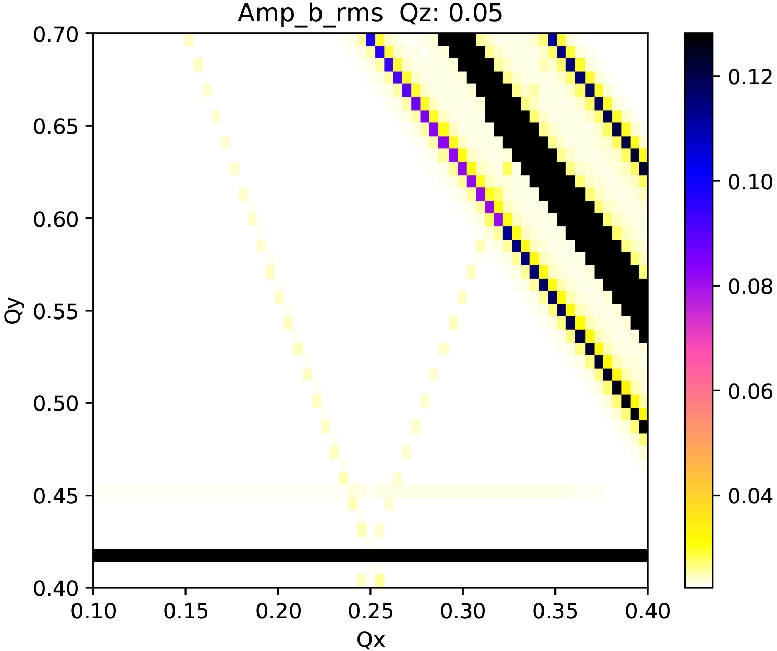
\includegraphics[width=\textwidth]{ts_plot1.pdf}
    \caption{2D density plot of the amp_b_rms data.}
    \label{f:plot1}
  \end{subfigure}
  \hfil
  \begin{subfigure}[t]{0.49\textwidth}
    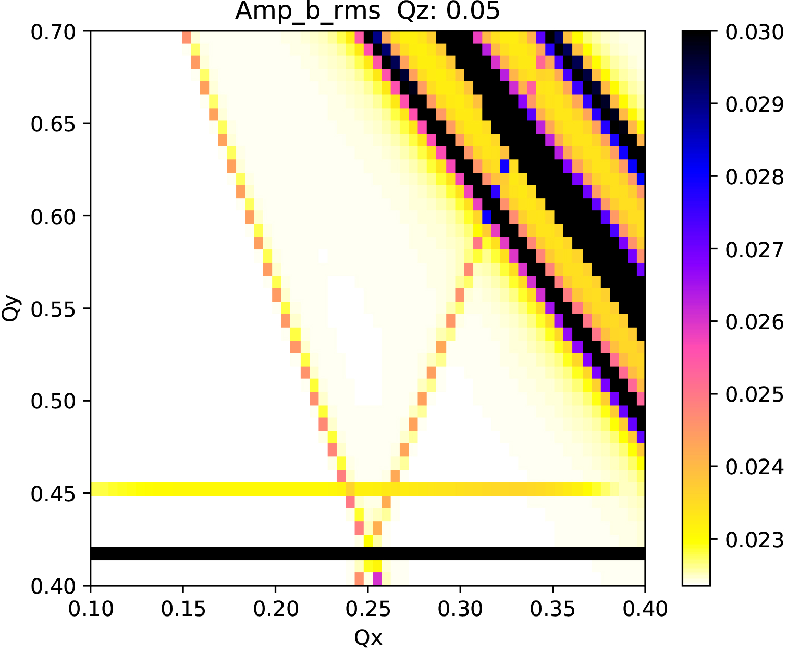
\includegraphics[width=\textwidth]{ts_plot2.pdf}
    \caption{2D density plot like \ref{f:plot1} with the range maximum reduced to 0.03.}
    \label{f:plot2}
  \end{subfigure}
  \caption{}
  \label{f:plot}
\end{figure}

%------------------------------------------------------------------
\Section{Plotting}
\label{s:plot}

There is a script named \vn{tune_scan_density_plot.py} for 2D density plotting of a tune plane data
set using Python. This script is in the directory (relative to the root of a Bmad Distribution)
\begin{code}
bsim/tune_scan/plotting
\end{code}
Example plots are in Fig.~\ref{f:plot}. 

The syntax for running the script is
\begin{code}
tune_plane_density_plot.py {-cmap <color_map>} {-column <col_to_plot>} 
            {-min <min_val>} {-max <max_val>} {-z <z_index>} {<data_file_name>}
\end{code}
Example:
\begin{code}
det_pix_plot.py -column 9 -max 0.05 -z 1 this_run.dat
\end{code}

\begin{description}
\item[<color_map>] \Newline
A \vn{color map} maps data values to the colors used in plotting. The underlying plotting package is called
\vn{matplotlib} and this package has a number of color maps which may be used. The default is \vn{gnuplot2_r}.
For a list of possible color maps, google ``matplotlib color maps''.
%
\item[<col_to_plot>] \Newline
Setting the column index \vn{<col_to_plot>} sets the column of data (\sref{s:out}) which is
plotted. Columns are numbered starting from zero so the column index of the \vn{amp_a_rms} data is column 7
and the \vn{amp_z_max} data is column 12.
%
\item[<min_val>, <max_val>] \Newline
minimum and maximum values for the data range to map onto the color map. Default values are the
minimum and maximum data values. Any datum values lower than the range minimum are set to the range
minimum and any datum values greater than the range maximum are set to the range maximum. This is useful
to emphasize features. For example, Fig.~\ref{f:plot2} is similar to Fig.~\ref{f:plot1} except the range
maximum has been reduced to 0.03. This better shows the weaker resonance lines.
%
\item[<data_file_name>] \Newline
The name of the data file. Default is \vn{tune_scan.dat}.
\end{description}

%------------------------------------------------------------------
\begin{thebibliography}{9}

\bibitem{b:bmad}
D. Sagan,
``Bmad: A Relativistic Charged Particle Simulation Library''
Nuc.\ Instrum.\ \& Methods Phys.\ Res.\ A, {\bf 558}, pp 356-59 (2006).

\end{thebibliography}

\end{document}

